\documentclass[svgnames,11pt]{standalone}
\usepackage[utf8]{inputenc}
\usepackage[T1]{fontenc}
\usepackage{csquotes}
\usepackage[english]{babel}
\usepackage{xcolor}
\usepackage{charter}
\usepackage{amsmath}
\usepackage{amssymb}
\usepackage[np,autolanguage]{numprint}
\newcommand{\outqt}[1]{{\textcolor{DarkOrange}{#1}}}
\newcommand{\inqt}[1]{{\textcolor{Blue}{#1}}}
\usepackage{tikz}
\usetikzlibrary{arrows,automata,calc}
\usetikzlibrary{arrows.meta}
\usetikzlibrary{decorations.pathreplacing}
\usetikzlibrary{backgrounds,shapes}
\tikzset{%
  show curve controls/.style={
    postaction={
      decoration={
        show path construction,
        curveto code={
          \draw [blue] 
            (\tikzinputsegmentfirst) -- (\tikzinputsegmentsupporta)
            (\tikzinputsegmentlast) -- (\tikzinputsegmentsupportb);
          \fill [red, opacity=0.5] 
            (\tikzinputsegmentsupporta) circle [radius=.25ex]
            (\tikzinputsegmentsupportb) circle [radius=.25ex];
        }
      },
      decorate
}}}
\tikzstyle{vertex}=[draw,circle,black,inner sep=2pt]
\tikzstyle{edge}=[line width=1.3pt,color=Black]
\tikzstyle{rare}=[fill=black,text=white]
\tikzstyle{medium}=[fill=black!15!white]


\begin{document}
  \tikzstyle{star}=[DodgerBlue,line width=1.7pt]
  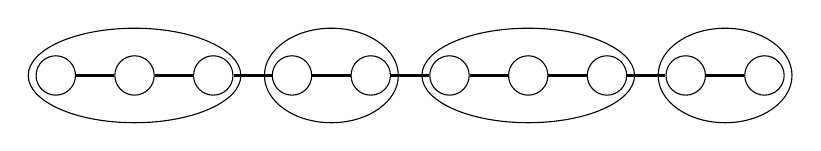
\begin{tikzpicture}[auto,vertex/.append style={minimum width=5mm},
    edge/.append style={line width=1.3pt,color=Black}]
    \node[vertex,] (p0) at (0.000,0.000) {};
    \node[vertex,] (p1) at (1.000,0.000) {};
    \draw[edge,] (p0) edge [bend left =0] node[] {} (p1);
    \node[vertex,] (p2) at (2.000,0.000) {};
    \draw[edge,] (p1) edge [bend left =0] node[] {} (p2);
    \node[vertex,] (p3) at (3.000,0.000) {};
    \draw[edge,] (p2) edge [bend left =0] node[] {} (p3);
    \node[vertex,] (p4) at (4.000,0.000) {};
    \draw[edge,] (p3) edge [bend left =0] node[] {} (p4);
    \node[vertex,] (p5) at (5.000,0.000) {};
    \draw[edge,] (p4) edge [bend left =0] node[] {} (p5);
    \node[vertex,] (p6) at (6.000,0.000) {};
    \draw[edge,] (p5) edge [bend left =0] node[] {} (p6);
    \node[vertex,] (p7) at (7.000,0.000) {};
    \draw[edge,] (p6) edge [bend left =0] node[] {} (p7);
    \node[vertex,] (p8) at (8.000,0.000) {};
    \draw[edge,] (p7) edge [bend left =0] node[] {} (p8);
    \node[vertex,] (p9) at (9.000,0.000) {};
    \draw[edge,] (p8) edge [bend left =0] node[] {} (p9);

    \draw[star] (p1) ellipse [x radius=1.35,y radius=.6];
    \draw[star] (3.5,0) ellipse [x radius=0.85,y radius=.6];
    \draw[star] (p6) ellipse [x radius=1.35,y radius=.6];
    \draw[star] (8.5,0) ellipse [x radius=0.85,y radius=.6];
  \end{tikzpicture}
\end{document}
